\documentclass[12pt, xcolor=dvipsnames]{scrartcl}

% include packages
% sonderzeichen encoding
% sonderzeichen encoding
\usepackage[utf8]{inputenc}
\usepackage[T1]{fontenc}
\usepackage[ngerman]{babel}

% xcolor package
\usepackage[dvipsnames,table]{xcolor}

% tables package & alternierende rowcolors in Tabellen
% alternating rowcolors in tables
\usepackage{longtable}
\rowcolors{2}{gray!15}{white}

% bilder
% bilder
\usepackage{graphicx}

% pdf includes
% pdf includes
\usepackage{pdfpages}

% toc als links rendern
% toc als links rendern
\usepackage[hidelinks]{hyperref}

% listings (source code)
%listing (source code)
\usepackage{listings}
\lstdefinelanguage{JavaScript}{
  keywords={typeof, new, true, false, catch, function, return, null, catch, switch, var, if, in, while, do, else, case, break},
  keywordstyle=\color{blue}\bfseries,
  ndkeywords={class, export, boolean, throw, implements, import, this},
  ndkeywordstyle=\color{darkgray}\bfseries,
  identifierstyle=\color{black},
  sensitive=false,
  comment=[l]{//},
  morecomment=[s]{/*}{*/},
  commentstyle=\color{purple}\ttfamily,
  stringstyle=\color{red}\ttfamily,
  morestring=[b]',
  morestring=[b]"
}

\lstset{
   language=JavaScript,
   backgroundcolor=\color{lightgray!50},
   extendedchars=true,
   basicstyle=\footnotesize\ttfamily,
   showstringspaces=false,
   showspaces=false,
   numbers=left,
   numberstyle=\footnotesize,
   numbersep=9pt,
   tabsize=2,
   breaklines=true,
   showtabs=false,
   captionpos=b
}

% show lof and lot in toc
% show lof and lot in toc
\usepackage[nottoc]{tocbibind}

% appendix
% appendix package
\usepackage[toc,page]{appendix}

% deutscher appendix name
\addto\captionsngerman{\let\appendixtocname\appendixname%
\let\appendixpagename\appendixname}

% nomencl (Abkuerzungsverzeichnis)
\usepackage[intoc]{nomencl}
\let\abbrev\nomenclature
\renewcommand{\nomname}{Abk\"urzungsverzeichnis}
\setlength{\nomlabelwidth}{7em}
\renewcommand{\nomlabel}[1]{#1 \dotfill}
\setlength{\nomitemsep}{-\parsep}

% einr�ckung for nomenclature
\usepackage{xstring}
\usepackage{xpatch}
\patchcmd{\thenomenclature}
  {\leftmargin\labelwidth}
  {\leftmargin\labelwidth\itemindent 1em }
  {}{}

\newcommand{\nomenclheader}[1]{%
  \item[\hspace*{-\itemindent}\normalfont\bfseries#1]}


\makenomenclature 

% ben�tigt f�r float angaben an tables, z.B. \begin{tyble}[H]
\usepackage{float}


% ben�tigt f�r \being{savenotes}, um fu�noten in tabellen zu verwenden
\usepackage{footnote}

% eurozeichen
\usepackage{eurosym}
\usepackage{textcomp}
\usepackage{amstext} % for \text
\DeclareRobustCommand{\officialeuro}{%
  \ifmmode\expandafter\text\fi
  {\fontencoding{U}\fontfamily{eurosym}\selectfont e}}


% used for linebreaks in table cells
\usepackage{pbox}

% amsmath, f�r aligned environment
\usepackage{amsmath}

% images in header & footer
% images in header & footer
% images in header & footer
\usepackage{fancyhdr}
\pagestyle{fancy}
\rhead{
\includegraphics[width=2cm]{images/gns}}


% keine einrück für neue absätze
\setlength{\parindent}{0pt}

% benötigt für float angaben an tables, z.B. \begin{tyble}[H]
\usepackage{float}

% benötigt für \being{savenotes}, um fußnoten in tabellen zu verwenden
\usepackage{footnote}


% eurozeichen
\usepackage{eurosym}
\usepackage{textcomp}
\usepackage{amstext} % for \text
\DeclareRobustCommand{\officialeuro}{%
  \ifmmode\expandafter\text\fi
  {\fontencoding{U}\fontfamily{eurosym}\selectfont e}}

% used for linebreaks in table cells
\usepackage{pbox}

\begin{document}


\newcommand{\Projekt}{Erstellung einer Webanwendung
		zur Verbesserung des Workflows des Erstellens von Benutzerhandbüchern}

\thispagestyle{empty}

\begin{center}
	\huge \bfseries
	Projektberich: \Projekt \\[4cm]

	\Large	\mdseries

	\textbf{Auszubildender} \\
	Oliver Herrmann \\
	Geb.: 23.09.1992 \\
	GNS mbH \\
	Tel.: +49 201 109 - 1523 \\
	Email: \href{mailto:oliver.herrmann@gns.de}{oliver.herrmann@gns.de}  \\
	Ausbildungsberuf: Fachinformatiker Anwendungsentwicklung \\[2cm]

	\textbf{Ausbildungsbetrieb} \\
	GNS mbH \\
	Frohnhauser Str. 67 \\
	45127 Essen \\[3cm]

	\today, Essen
\end{center}



\clearpage

\tableofcontents
\clearpage

\listoffigures
\clearpage

\listoftables
\clearpage

\abbrev{KIS}{Abteilung der GNS für Softwareentwicklung}
\abbrev{GNS}{Gesellschaft für Nuklear-Service mbH}	
\abbrev{Hosting}{Bereitstellen einer Web-Anwendung auf einem Web-Server}	
\abbrev{CVS}{Concurrent Version System}	
\printnomenclature		
\clearpage



\section{Einleitung}

\subsection{Projektumfeld}
\label{sec:projektumfeld}

Die GNS (Gesellschaft für Nuklear-Service) mbH ist ein mittelständisches Unternehmen, das 1977 gegründet wurde und aktuell etwa 550 Mitarbeiter beschäftigt. Die Firmenzentrale befindet sich in Essen. Die GNS betreibt des weiteren Standorte in Duisburg, Mülheim an der Ruhr und Karlsruhe. Das Hauptgeschäftsfeld der GNS ist die Entwicklung sowie der Vertrieb von Behältern zur Lagerung und zum Transport von radioaktivem Material, als auch die Beladung solcher Behältnisse.


Ebenfalls zum Geschäftsbereich der GNS zugehörig ist der Ver- und Betrieb von Softwarelösungen. Hier ist beispielhaft das AVK(Abfallfluss- Verfolgungs- und Produktkontroll-System) zu nennen, welches 1991 entwickelt wurde und heute in allen deutschen Kernkraftwerken verwendet wird.  Daneben werden von der GNS eine Vielzahl von stark spezialisierten Softwarelösungen betrieben, wovon viele als digitale Dienstleistung für Kunden (z.B. Kernkraftwerke und Zwischenlager) bereitgestellt werden. \\

Auftraggeber des Projekts ''\Projekt'' ist die GNS, in Person Friedrich Bauriedel, Leiter der Abteilung KIS.



\subsection{Projektziel}

Ziel des Projekts ist, den regelmäßig anfallenden Arbeitsschritt ''Erstellen eines Benutzerhandbuch aus einem Wiki'' für die Mitarbeiter der GNS zu vereinfachen und zu beschleunigen. Ebenfalls soll der Workflow normiert und zentralisiert werden, sodass der Aufwand für vorlaufende Arbeiten minimiert wird.

\subsection{Projektbegründung}
\label{sec:projektbegründung}

Wie in \ref{sec:projektumfeld} erwähnt betreibt die GNS eine Vielzahl an hoch spezialisierten Softwarelösung für diverse Kunden. Aufgrund der Komplexität vieler dieser Anwendungen ist es nötig den Benutzern ein Handbuch zur Verfügung zu stellen.
Zu diesem Zweck betreibt die GNS betriebsinterne Wikis, in denen Inhalte bezüglich der korrekten Bedienung einer Anwendung von Mitarbeitern der GNS gepflegt werden. \\

2012 wurde von der GNS der sogenannte WikiConverter entwickelt. Dies ist ein Tool, welches die Inhalte eines MediaWikis extrahiert und diese in ein PDF- bzw. ein HTML-Dokument konvertiert.
Ziel der Entwicklung war es, die mithilfe des WikiConverters erzeugten Dateien als interaktive Hilfe in die jeweiligen Anwendungen einzubetten bzw. als Benutzerhandbuch den Kunden bereitstellen zu können.

Allerdings wurde bei der Entwicklung des WikiConverters wenig Wert auf eine intuitive Benutzerführung gelegt, was dazu führte, dass die Bedienung von diesem äußerst komplex ist. \\

Durch die in den letzten Jahren gesteigerte Anzahl der von der GNS betriebenen Softwarelösungen, sowie die stetige Verkürzung der Release-Intervalle dieser, ist der Arbeitsschritt ''Erstellen von Benutzerhandbüchern'' immer mehr in den Vordergrund gerückt, was schließlich dazu führte, dass eine Überarbeitung von diesem unumgänglich wurde. \\

Zu diesem Zweck wurde von der Abteilung KIS Mitte 2015 das Projekt ''\Projekt'' initiiert, welches zum Ziel hat, die Erstellung von Benutzerhandbüchern zu vereinfachen und zu zentralisieren.

Im Rahmen des Projekts wird eine Web-Anwendung entwickelt, welche die Kernfunktionalität des WikiConverters ummantelt und eine einheitliche, graphische Benutzerschnittstelle zu dieser anbietet. So wird die Komplexität des WikiConverters vor den Benutzern verborgen, um diesen eine einfachere und intuitivere Benutzung zu ermöglichen. \\

Als messbares Ziel des Projekts ist eine Reduzierung der durchschnittlichen Arbeitszeit für den Workflow ''Erstellen eines Benutzerhandbuchs'' um mindestens 25\% veranschlagt.


\subsection{Projektschnittstellen}

Die technischen und sozialen Schnittstellen des Projekts sind ausschließlich betriebsinterner Natur. \\
Technisch betrachtet greif das Projekt die bestehende Anwendung ''Wikiconverter'' auf und adaptiert dessen Kernfunktionalität. \\
Aus projekt-spezifischer Sicht sind die Schnittstellen rein intern, da sowohl Auftraggeber als auch Endnutzer der Anwendung Mitarbeiter bzw. Abteilungen der GNS sind. \\
Die Projektabschließende Abnahme erfolgt gegenüber dem Auftraggeber, hier die Abteilung KIS der GNS.


\subsection{Projektabgrenzung}

Ausdrücklich nicht Teil des Projekts ist das Hosting der im Rahmen des Projekts entwickelten Anwendung sowie alle in Verbindung mit dem Hosting stehenden administrativen Maßnahmen. Diese werden von nicht direkt am Projekt beteiligten Mitarbeitern der GNS durchgeführt.


\section{Projektplanung}

\subsection{Projektphasen}

	\begin{table}[H]
	\centering
	\begin{tabular}{lr}

		\rowcolor{MidnightBlue!15}				
		\textbf{Projekphase} & \textbf{Geplante Zeit} \\\hline
		
	    Anforderungsanalyse & 7h \\	   	   
	    Projektplanung & 4h \\	   			
	    Software-Architektur & 14h \\	 				
	    Implementierung & 26h \\	   				
	    Projektabschluss & 3h \\	   				
	    Sonstiges & 16h \\\hline
	  		
		\rowcolor{MidnightBlue!15}				
		\textbf{Gesamt} & \textbf{70h}				
			    
	\end{tabular}
	\caption{Projektphasen}
	\label{tab:projektphasen}
	\end{table}
	
	Eine detaillierte Übersicht der einzelnen Phasen findet sich im Anhang \ref{app:projektphasen_detail} auf Seite \pageref{app:projektphasen_detail}
	

\subsection{Abweichung vom Projektantrag}

Abweichend vom Projektantrag werden das Pflichten- sowie das Lastenheft nur in Auszügen im Projektbericht aufgeführt. Dies geschieht aus dem Grund den Umfang des Projektbericht nicht übermäßig zu gestalten.

\subsection{Resourcenplanung}

Im Folgenden werden alle für die Durchführung des Projekts bezogenen Resourcen aufgelistet. Diese werden durch den Auftraggeber, hier die GNS, bereitgestellt.

\begin{table}[H]
	\centering
	\begin{tabular}{ll}

		\rowcolor{white!15}				
		\textbf{Art der Resource} & \textbf{Beschreibung} \\\hline		
		
		\rowcolor{MidnightBlue!15}				
		\textbf{Sachliche Resource} & \\
		Projektbüro & \\
		Computer & \\
		\hspace{1.5em} IDE & Eclipse for JEE Developers \\
		Demilitarisierte Zone & zu Testzwecken \\
		
		\rowcolor{MidnightBlue!15}			
		\textbf{Personelle Resource} & \\
		Projektleiter & Oliver Herrmann \\
		Projektmitarbeiter & Oliver Herrmann \\
	
			    
	\end{tabular}
	\caption{Projektphasen}
	\label{tab:projektphasen}
	\end{table}

\subsection{Entwicklungsprozess}

Grundlage für den Entwicklungsprozess bildet das iterative Wasserfallmodell\footnote{\url{http://www.pi.informatik.tu-darmstadt.de/fileadmin/user_upload/Group_PI/LV__SE_RE/R_01_Wasserfallmodell__Ausarbeitung__Schwaiger.pdf} abgerufen am 05.10.2015}.
Dies wurde vor allem gewählt, da es gut mit Projekten geringen bis mittleren Umfangs harmoniert. Andere Modelle wie z.B. Scrum oder Extreme-Programming wurden in erster Linie nicht gewählt, da diese die Projektarbeit in einem Team erfordern.

\section{Analysephase}

\subsection{Ist-Analyse}

Der jetzige Stand bezüglich des Workflows ''Erstellen eines Benutzerhandbuch'' sieht vor, dass der ausführende Mitarbeiter den WikiConverter aus dem internen CVS auscheckt, im Quellcode angaben zu dem zu konvertierenden Wiki (URL, Hauptseite) ergänzt und den Quellcode anschließende kompiliert und ausführt. Das Ergebnis der Ausführung sind die generierten PDF- und HTML-Dateien.

Das Projekt ''\Projekt'' sieht vor, den Workflow wie folgt zu definieren:
\begin{itemize}
	\item Der Benutzer loggt sich online in der Anwendung ein.
	\item Der Benutzer wählt ein existierendes Wiki aus oder pflegt ein neues ein. (Nötige Angaben sind URL und Hauptseite des Wikis)
	\item Der Benutzer kann über die graphische Oberfläche das Konvertieren starten.
	\item Nach erfolgreicher Konvertierung kann der Benutzer die generierten Dateien herunter laden.
\end{itemize}

Außerdem werden aus Konvertierungsvorgängen erstellte Dateien dauerhaft gespeichert. Diese können ebenfalls vom Benutzer heruntergeladen werden, falls eine neue Konvertierung nicht benötigt wird.

\subsection{Wirtschaftlichkeitsanalyse}
\label{sec:wirtschaftlichkeitsanalyse}

Im folgenden wird die Wirtschaftlichkeit des Projekts betrachtet. Da das Projekt keinen direkten Gewinn erwirtschaftet sondern der monetäre Vorteil durch die Erleichterung der Arbeit der betroffenen Mitarbeiter erzielt wird, wird zuerst der Nutzen des Projekts messbar festgehalten. Dieser wird dann den Kosten des Projekts gegenübergestellt um eine qualifizierte Aussage über die Wirtschaftlichkeit des Projekt zu machen.

Grundlage der Analyse sind folgende Stundensätze\footnote{Beruhend auf Schätzungen bzw. betriebsinternen Angaben}:

\begin{table}[H]
	\centering
	\begin{tabular}{lr}

		\rowcolor{white!15}				
		\textbf{Art der Beschäftigung} & \textbf{Stundensatz} \\\hline		
		
		Fachinformatiker & 30 \euro \\
		Auszubildender & 7 \euro \\
		Gemeinkosten & 10 \euro \\
			    
	\end{tabular}
	\caption{Stundensätze}
	\label{tab:stundensätze}
\end{table}

Hieraus ergibt sich ein \textit{effektiver} Stundensatz von 30 \euro{} für die Arbeit eines Fachinformatikers, bzw. 17 \euro{} für die Arbeits eines Auszubildenden (hier Projektmitarbeiter).


\subsubsection{Nutzen des Projekts}
\label{sec:nutzen_des_projekts}

Der Nutzen des Projekts manifestiert sich primär darin, dass der regelmäßig auftretende Workflow ''Erstellen eines Benutzerhandbuchs'' beschleunigt wird.
Da die exakte Bestimmung der durchschnittlich für diesen Workflow anfallenden Zeit von vielen, auch personellen, Faktoren abhängt, wird er für die Zwecke der Wirtschaftlichkeitsanalyse konservativ abgeschätzt. Diese Schätzung wird fortan als Grundlage für weitere Berechnungen herangezogen, um so ein Worst-Case Ergebnis ausdrücken zu können.
Der aktuelle durchschnittliche zeitliche Aufwand für den Workflow ergibt sich aus
\begin{itemize}
	\item Einarbeitung in den Workflow und den WikiConverter im Allgemeinen
	\item Auschecken der Quellen
	\item Anpassungen am Quellcode
	\item Kompilieren der Quellen
	\item Ausführen der Anwendung
	\item Sichern der Ergebnisse
\end{itemize}
und beträgt nach Schätzungen \textbf{8 Minuten}. \\

Der neue, vom Projekt angestrebte Workflow setzt sich dagegen wie folgt zusammen \\

Alternative 1
\begin{itemize}
	\item Login
	\item Konvertierung anstoßen
	\item herunterladen der Ergebnisse
\end{itemize}
Geschätze Dauer: 5 Minute. \\

Alternative 2
\begin{itemize}
	\item Login
	\item Auswählen eines bereits existierenden Ergebnisses
	\item herunterladen der Ergebnisse
\end{itemize}
Geschätze Dauer: 2 Minuten. \\


Hier ist anzumerken, dass durch die zentrale Speicherung der konvertierten Ergebnisse dem Nutzer ermöglicht wird, den zeitintensiven Schritt der Konvertierung auszulassen, wenn ein adäquates Ergebnis bereits existiert. Dies ist z.B dann der Fall, wenn die Konvertierung kürzlich durch einen dritten Mitarbeiter vorgenommen wurde und seit dem keine relevanten Änderungen am zu Grunde liegenden Wiki auftraten.

Konservativ abgeschätzt wird davon ausgegangen, dass in 80\% der Fälle Alternative 1 und in den übrigen 20\% Alternative 2 eintreten wird.
\begin{equation} \label{eq:1}
	T_\emptyset = 0.8 * 5m + 0.2* 2m = 4.4m
\end{equation}

Aus Formel \ref{eq:1} ergibt sich eine durchschnittliche Dauer des Workflows von \textbf{4,4 Minuten}.



\begin{equation} \label{eq:2}
	T_\Delta = \frac{(8m-4,4m)}{8m} = 45\%
\end{equation}

Dies entspricht nach Formel \ref{eq:2} einer Einsparung von \textbf{45\%} und verspricht ein Einhalten des in Kapitel \ref{sec:projektbegründung} ausgesprochenen Ziels, die durchschnittliche Arbeitszeit des Workflows um mindestens mindestens 25\% zu reduzieren. \\

\begin{equation} \label{eq:3}
	K_{wöchtl} = 7,2m * \frac{1h}{60m} * \frac{40 \euro}{h} = 4,8 \euro
\end{equation}

Unter der Annahme, dass der Workflow durchschnittlich zweimal pro Woche durchgeführt wird ergibt sich daraus eine Zeitersparnis von 7,2m pro Woche, was nach Formel \ref{eq:3} einer wöchentlichen monetären Ersparnis von \textbf{4,8 \euro{}} entspricht.


\subsubsection{Kosten des Projekts}
\label{sec:kosten_des_projekts}

Die Kosten des Projekts werden allein durch die Kosten der Entwicklung bestimmt. Es werden keine nicht bereits vorhandenen Ressourcen für das Projekt verwendet.
\begin{equation} \label{eq:4}
	K_{ges} = 70h * \frac{17 \euro}{h} = 1190 \euro
\end{equation}
Bei einem kalkulierten Projektumfang von 70 Stunden ergibt sich aus Formel \ref{eq:4} ein Kostenumfang von \textbf{1190 \euro{}}, unter der Voraussetzung, dass als Projektmitarbeiter ausschließlich Auszubildende eingesetzt werden.


\subsubsection{Wirtschaftlichkeit des Projekts}
Zieht man die Ergebnisse aus Kapitel \ref{sec:nutzen_des_projekts} und \ref{sec:kosten_des_projekts} heran und betrachtet diese relativ zueinander, lässt sich feststellen, dass sich das Projekt in etwa 5 Jahren armortisiert hat.


\subsection{Risikoanalyse}

Im folgenden wird eine Risikoanalyse und -bewertung durchgeführt.
Eine detaillierte Übersicht der Risikobewertung findet sich im Anhang \ref{app:risikoanalyse} auf Seite \pageref{app:risikoanalyse}.

Zusammenfassend lässt sich das Ergebnis der Risikoanalyse in drei Teilbereiche gruppieren.

\paragraph{Gruppe 1}
Unvermeidbare Risiken \\
Hierzu zählen z.B. krankheitsbedingte personelle Ausfälle. Diese stellen ein unvermeidbares Risiko dar. Eine Strategie zur Vermeidung ist hier nicht vorgesehen.\\

\paragraph{Gruppe 2}
Bedingt vermeidbare Risiken \\
Hierzu zählen vor allem Risiken aus Fehlern der Planung. Diese Risiken sind bedingt vermeidbar. Dem Auftreten solcher Risiken wird insbesondere durch die im  Qualitätssicherungskonzept vorgesehenen Zwischenstandsanalysen entgegengewirkt.

\paragraph{Gruppe 3}
Leicht vermeidbare Risiken \\
Dies sind in erster Linie Risiken die in der Entwicklung auftreten können. Das Eintreten dieser Risiken wird in erster Linie durch die Erfahrung und intensive fachliche Vorbereitung der Projektmitarbeiter vermieden. Des weiteren hilft das im Qualitätssicherungskonzept beinhaltete Testkonzept hier für eine frühzeitige Erkennung von Konsequenzen dieser Risikogruppe.


Die möglichen Konsequenzen lassen sich wiederum in zwei Bereiche gruppieren.

\paragraph{Gruppe A} Zeitliche Konsequenzen \\
Dies sind Risikofolgen, welche in erster Linie eine Ausdehnung des Projektzeitraums bzw. eine Verzögerung des Projektabschlusses mit sich ziehen. Da das Projekt allerdings für rein betriebsinterne Zwecke konzipiert ist und keinen direkten Gewinn erwirtschaftet beschränken sich die negativen Auswirken dieser Gruppe auf ein Minimum. Dies hat zur Folge, dass Zeitliche Konsequenzen, sofern sie nicht in sehr hoher Quantität auftreten, nicht zum Abbruch des Projekts führen.

\paragraph{Gruppe B} Finanzielle Konsequenzen \\
Dies sind Risikofolgen, welche primär eine Erhöhung des monetären Aufwands des Projekts mit sich ziehen. Erzeugt werden diese Konsequenzen vor allem durch Verzögerungen im Projektablauf.

Da das Projektbudget ausschließlich für die Beschäftigung der Projektmitarbeiter aufgewendet wird, ergibt sich dessen Betrag aus der geplanten Projektdauer. Dies hat zur Folge, dass finanzielle Konsequenzen direkt mit zeitlichen Konsequenzen gleichgesetzt werden können und daher, bei gemäßigten Auftreten, nicht zum Projektabbruch führen.


\subsection{"Make or Buy"-Entscheidung}

Im Folgenden wird abgewägt, ob sich das Projekt bezüglich Nutzen und Wirtschaftlichkeit gegenüber bereits existierenden Lösungen behauptet.


\begin{table}[H]
	\centering
	\begin{tabular}{lcc}

		\rowcolor{white!15}				
		\textbf{Alternative} & \textbf{Nutzen} & \textbf{Wirtschaftlichkeit} \\\hline		
				
		MediaWiki Erweiterung & $\ominus\ominus\ominus$ & $\ominus\ominus\ominus\ominus$ \\		
		Erstellung der Anwendung durch Dienstleister & $\oplus\oplus$ & $\ominus\ominus\ominus$ \\		
		Eigenständige Erstellung der Anwendung & $\oplus\oplus\oplus$ & $\ominus\ominus$ \\
	
			    
	\end{tabular}
	\caption{"Make or Buy"-Bewertung}
	\label{tab:make_or_buy}
\end{table}

Eine detaillierte Übersicht der ''Make or Buy''-Bewertung findet sich im Anhang \ref{app:make_or_buy} auf Seite \pageref{app:make_or_buy}.


Als Ergebnis der ''Make or Buy''-Analyse lässt sich festlegen, dass eine eigenständige Entwicklung der Anwendung aus wirtschaftlicher und nutzenorientierter Sicht die beste Alternative darstellt.


\subsection{Projektkosten}

Wie in Kapitel \ref{sec:kosten_des_projekts} bereits erläutert setzen sich die Kosten ausschließlich aus den Mitarbeiterkosten der Projektmitarbeiter zusammen. Da für das Projekt nur ein Mitarbeiter veranschlagt ist, sind die Kosten äquivalent zu der kalkulierten Dauer des Projekts.

\begin{equation} \label{eq:5}
	K_{ges} = T_{ges} * K_{proj_mitarbeiter} = 70h * \frac{17 \euro}{1h} = 1190 \euro
\end{equation}

Aus Formel \ref{eq:5} wird ersichtlich, dass sich die Gesamtkosten des Projekts auf \textbf{1190 \euro{}} belaufen.

Eine detaillierte, nach Phasen unterteilte Übersicht der Kosten findet sich im Anhang \ref{app:kosten} auf Seite \pageref{app:kosten}

\subsection{Amortisationsdauer}

Siehe Kosten und Nutzen

\subsection{Nutzwertanalyse}

Für die entwicklungsrelevanten Bereiche ''Backend'' und ''Frontend'' werden jeweils Nutzwertanalysen durchgeführt, um im Vorhinein die optimale Architektur zu bestimmen.

\begin{table}[H]
	\centering
	\begin{tabular}{ll}

		\rowcolor{white!15}				
		\textbf{Architekturbereich} & \textbf{beste Alternative} \\\hline		
				
		Backend & JEE-Stack \\
		Frontend & HorCrux	\\	
			    
	\end{tabular}
	\caption{Ergebnis der \nameref{app:nutzwertanalyse}}
	\label{tab:nutzwertanalyse}
\end{table}

Die zugrunde liegenden Nutzweranalysen befinden sich im Anhang \ref{app:nutzwertanalyse} auf Seite \pageref{app:nutzwertanalyse}.

\subsection{Anwendungsfälle}

Die Anwendung deckt alle für den Workflow ''Erstellen eines Handbuchs'' relevanten Anwendungsfälle ab. Auch vor- und nachbereitende Anwendungsfälle werden von der Anwendung abgedeckt.

Es folgt eine Auflistung aller relevanten Anwendungsfälle.

\begin{enumerate}
	\item vorgelagerte Anwendungsfälle
	\begin{enumerate}
		\item Anlegen eines Benutzers		
		\item Login durch einen Benutzer
		\item Anlegen eines neues Wikis	
	\end{enumerate}
	\item Hauptanwendungsfälle
	\begin{enumerate}
		\item Konvertieren eines Wikis \label{item:wiki_konvertieren}
		\item Herunterladen eines Konvertierungsergebnisses
		\item Bearbeiten eines Wikis \label{item:wiki_bearbeiten}
	\end{enumerate}
	\item nachgelagerte Anwendungsfälle
	\begin{enumerate}
		\item Löschen eines Benutzers
		\item Löschen eines Wikis
		\item Löschen eines eines Konvertierungsergebnisses
	\end{enumerate}
\end{enumerate}

Zu den Anwendungsfällen \ref{item:wiki_konvertieren} und \ref{item:wiki_bearbeiten} finden sich im Anhang \ref{app:use_case_diagramm} auf Seite \pageref{app:use_case_diagramm} Use-Case-Diagramme, welche die Anwendungsfälle detailliert darstellen.


\subsection{Qalitätsanforderungen}

\subsection{Lastenheft / Fachkonzept}

\subsection{Zwischenstand}

\section{Entwurfsphase}

\subsection{Zielplattform}

\subsection{Architekturdesign}

\subsection{Entwurf der Benutzeroberfläche}

\subsection{Datenmodell}

\subsection{Geschäftslogik}

\subsection{Maßnahmen zur Qualitätssicherung / Testkonzept}

\subsection{Pflichtenheft / Datenverarbeitungskonzept}

\subsection{Zwischenstand}

\section{Implementierungsphase}

	Hier erfolgen Details über die Implementierung

\subsection{Implementierung der Datenstruckturen}

\subsection{Implementierung des Backends}

\subsection{Implementierung des Frontends}

\subsection{Implementierung der Tests}

\subsection{Zwischenstand}

\section{Abnahmephase}
	test

\subsection{Zwischenstand}

\section{Einführungsphase}

\subsection{Zwischenstand}


\section{Dokumentation}

\subsection{Zwischenstand}

\section{Fazit}

\subsection{Soll- / Ist-Vergleich}

\subsection{Lesson-Learned}

\subsection{Ausblick}

\newpage

% \inputencoding{utf8}

\begin{appendices}
% \renewcommand{\thesection}{\arabic{section}} %\Roman{section}

\addtocontents{toc}{\protect\setcounter{tocdepth}{1}}
	
	\section{Projektphasen}		
		\label{app:projektphasen_detail}
\begin{table}[H]
	\centering
	\begin{tabular}{lr}

		\rowcolor{white!15}				
		\textbf{Projekphase} & \textbf{Geplante Zeit} \\\hline

		\rowcolor{MidnightBlue!25}
	    Anforderungsanalyse & Gesamt: 7h \\\hline
	    Sichtung des Lastenhefts & 1h \\	    
	    Erstellen des Pflichtenhefts & 2h \\	    
	    Wirtschaftlichkeitsanalyse & 1h \\	     
	    Risikoanalyse & 1h \\	      
	    ''Make or Buy'' Analyse & 1h \\	    
		Anwendungsfälle definieren & 1h \\

	    \rowcolor{MidnightBlue!25}
	    Projektplanung & Gesamt: 4h \\\hline
	    Erstellen des Projektplans & 2h \\
		Erstellen des Qualitätssicherungskonzepts & 2h \\
		
		\rowcolor{MidnightBlue!25}
	    Software-Architektur & Gesamt: 14h \\\hline
	    Spezifizieren der Architekturgrundlagen & 8h \\
		Erstellen des Datenmodells & 4h \\
		Erstellen des Testkonzepts & 2h \\
		
		\rowcolor{MidnightBlue!25}
	    Implementierung & Gesamt: 26h \\\hline
	    Erstellen der Datenbanktabellen & 2h \\
		Entwicklung des Backends & 7h \\
		Entwicklung des Frontends & 9h \\
		Dokumentation des Quellcodes & 2h \\
	    Testing & 2h \\
		Soll-Ist-Vergleich & 2h \\
		Puffer für Korrekturen & 2h \\
		
		\rowcolor{MidnightBlue!25}
	    Projektabschluss & Gesamt: 3h \\\hline
	    Anwenderschulung & 2h \\
		Abnahme & 1h \\
		
		\rowcolor{MidnightBlue!25}
	    Sonstiges & Gesamt: 16h \\\hline
	    Projektdokumentation & 12h \\
		Allgemeiner Puffer & 4h \\\hline
		
		\textbf{Gesamt} & \textbf{70h}				
			    
	\end{tabular}
	\caption{Projektphasen detailliert}
	\label{tab:projektphasen_detail}
	\end{table}
		\newpage

	\section{Risikoanalyse}		
		\label{app:risikoanalyse}

	\begin{longtable}{
		p{\dimexpr 0.2\linewidth-2\tabcolsep} |
		p{\dimexpr 0.2\linewidth-2\tabcolsep} |
		p{\dimexpr 0.2\linewidth-2\tabcolsep} |
		p{\dimexpr 0.2\linewidth-2\tabcolsep} |
		p{\dimexpr 0.2\linewidth-2\tabcolsep}
	}

		\rowcolor{white!15}				
		\textbf{Risiko} & \textbf{Ursache} & \textbf{Maßnahme} & \textbf{Eintrittswahr. nach der Maßnahme} & \textbf{Auswirkung nach der Maßnahme} \\\endhead\hline

	
		\rowcolor{MidnightBlue!25}
		\multicolumn{5}{c}{Terminrisiken} \\\hline
		Nicht einhalten des Abnahmetermins & uneingeplante Hindernisse & keine & mittel & Start der Anwendungsnutzung verzögert sich \\
		
		\rowcolor{MidnightBlue!25}
		\multicolumn{5}{c}{Technische Risiken} \\\hline
		Anwendung ist auf Zielplattform nicht lauffähig & Entwicklung gegen falsche Plattform & Anpassung der Anwendung & mittel & Zustäzlicher Zeitbedarf für Anpassungen \\
		
		\rowcolor{MidnightBlue!25}
		\multicolumn{5}{c}{Personelle Risiken} \\\hline
		Ausfall des Projektleiters & Krankheit & keine & gering & Projekt kommt zum erliegen \\		
		Ausfall eines Projektmitarbeiters & Krankheit & keine & gering & Projekt kommt zum erliegen \\
						
		\rowcolor{MidnightBlue!25}
		\multicolumn{5}{c}{Planungsrisiken} \\\hline
		Unterschätzung der Dauer einzelner Phasen & mangelnde Erfahrung & nachtrgäliche Planung & mittel & Verzögerung des Projektabschluss \\
		Auslassung relevanter Phasen & mangelnde Erfahrung & nachträgliche Planung & gering & Verzögerung des Projektabschluss \\
		
		\rowcolor{MidnightBlue!25}
		\multicolumn{5}{c}{Risiken der Analyse und Konzeption} \\\hline
		Fehlerhafte Ist-Analyse & ungenaue Analyse & Nachbesserung d. Analyse & gering & iterativer Rücksprung im Entwicklungsprozess \\
		Fehlerhafte Soll-Analyse & fehlerhafte Spezifikation & Nachbesserung d. Analyse & gering & iterativer Rücksprung im Entwicklungsprozess \\
		Fehlerhafte Architektur / Konzept & ungenaue Spezifikation & Neukonzeption & gering & iterativer Rücksprung im Entwicklungsprozess \\
		
		\rowcolor{MidnightBlue!25}
		\multicolumn{5}{c}{Realisierungrisiken} \\\hline
		Unerwartete Entwicklungsprobleme & nicht bestimmbar & teilweise NeuKonzeption & mittel & verlängte Entwicklungszeit \\
		
		\rowcolor{MidnightBlue!25}
		\multicolumn{5}{c}{Betreuungs- und Wartungsrisiken} \\\hline
		Breaking-Changes & MediaWiki Update & Anpassung der Geschäftslogik & hoch & keine \\
	    
	
	\caption{Risikoanalyse detailliert}
	\label{tab:risikoanalyse_detail}	
\end{longtable}
	

		\newpage		
		
	\section{''Make or Buy''-Bewertung}		
		\label{app:make_or_buy}

Grundlage der im Folgenden betrachteten Alternativen ist eine umfängliche Recherche bezüglich der Kernfrage
''Welche Lösungen zur Erstellung von Handbüchern aus Wikis existieren bereits?''.
Betrachtet werden hier nur die stärksten Ergebnisse dieser Recherche, um die Übersichtlichkeit der Analyse zu bewahren.

\begin{table}[H]
	\centering
	\begin{tabular}{lcc}

		\rowcolor{white!15}				
		\textbf{Alternative} & \textbf{Nutzen} & \textbf{Wirtschaftlichkeit} \\\hline		
		
		\rowcolor{MidnightBlue!15}
		MediaWiki Erweiterung 								& 					& 							\\\hline
		\hspace{1.5em} einfache Installation 				&					& $\oplus$  				\\
		\hspace{1.5em} Installation für jedes Wiki nötig 	&					& $\ominus$ 				\\
		\hspace{1.5em} Workflow umständlich 				& $\ominus$ 		& $\ominus$ 				\\
		\hspace{1.5em} Ergebnis bedarf händische Anpassung	& $\ominus\ominus$	& $\ominus\ominus$ 			\\
		\hspace{1.5em} Komptibilitätsprobleme mit MediaWiki	&  					& $\ominus$ 				\\
		
		\rowcolor{MidnightBlue!15}
		Erstellung der Anwendung durch Dienstleister 		& 					& 							\\\hline
		\hspace{1.5em} spezialisierte Anwendung 			& $\oplus\oplus$	& $\ominus\ominus\ominus$	\\
		\hspace{1.5em} Wartung durch Dienstleister nötig 	&					& $\ominus\ominus$ 			\\
		\hspace{1.5em} Risikoauslagerung 					&  					& $\oplus\oplus$ 			\\
		
		\rowcolor{MidnightBlue!15}
		Eigenständige Erstellung der Anwendung 				& 					& 							\\\hline
		\hspace{1.5em} spezialisierte Anwendung 			& $\oplus\oplus$	& $\ominus\ominus$ 			\\
		\hspace{1.5em} Wartung durch eigene Mitarbeiter  	& $\oplus$			& $\oplus$ 					\\
		\hspace{1.5em} Tragen von Risiken 					&  					& $\ominus$ 				\\									
			    
	\end{tabular}
	
	\caption{Detaillierte ''Make or Buy''-Bewertung}
	\label{tab:make_or_buy_detail}
\end{table}		
		\newpage
	
	\section{Kosten\"ubersicht nach Projektphasen}		
		\label{app:kosten}

Grundlage der Folgenden Kostenübersicht sind die in Anhang \ref{app:projektphasen_detail} aufgeführten Phasen des Projekts.
Als Rechnungsgrundlage wird der in Kapitel \ref{sec:wirtschaftlichkeitsanalyse} ermittelte Stundensatz von 17 \euro{} herangezogen.

\begin{table}[H]
	\centering
	\begin{tabular}{lr}

		\rowcolor{white!15}				
		\textbf{Phase} & \textbf{Kosten}  \\\hline		
		
		
		Anforderungsanalyse		& 119 \euro \\
		Projektplanung			& 68 \euro \\
		Software-Architektur	& 238 \euro \\
		Implementierung			& 442 \euro \\
		Projektabschluss		& 51 \euro \\
		Sonstiges				& 272 \euro \\\hline
		\textbf{Gesamt}			& \textbf{1190 \euro}
		
			    
	\end{tabular}
	
	\caption{Kosten unterteilt nach Projektphasen}
	\label{tab:kosten_detail}
\end{table}		
		\newpage

	\section{Nutzwertanalyse}		
		\label{app:nutzwertanalyse}

\subsubsection{Backend-Architektur}

Im Folgenden wird über eine Nutzwertanalyse die beste Backend-Architektur ausgewählt.
Die hier betrachteten Alternativen sind die stärksten Ergebnisse einer vorangegangen Recherche. 

\begin{savenotes}
\begin{table}[H]
	\centering
	\begin{tabular}{lcccc}

		\rowcolor{white!15}				
		\textbf{Eigenschaft} 			& \textbf{Gewichtung}
			& \textbf{JEE-Stack\footnote{\url{http://www.oracle.com/technetwork/java/javaee/overview/index.html}, abgerufen am 08.11.2015}}
			& \textbf{GNS-Framework\footnote{ein betriebsinternes Framework zur entwicklung von Webanwendungen}}
			& \textbf{SrpingMVC\footnote{\url{https://spring.io}, abgerufen am 08.11.2015}} \\\hline		
		
		REST-Api integriert				& 3						& 5						& 0							& 4 \\
		\pbox{4cm}{Trennung von \\ Back- und Frontend}	& 4						& 5						& 0							& 4 \\						
		Dokumentation					& 2						& 3						& 1							& 5 \\
		Testbarkeit						& 2						& 2						& 1							& 3 \\
		\pbox{4cm}{Refactoring \\(ggf. durch Dritte)}	& 3						& 3						& 4							& 2 \\
		
		\rowcolor{MidnightBlue!15}
		\textbf{Gesamt}				& \textbf{14}			& \textbf{18}			& \textbf{6}				& \textbf{18} \\\hline
		\rowcolor{white!15}				
		\textbf{Nutzwert} 				& 						& \textbf{3,86}			& \textbf{1,14} 			& \textbf{3,57} \\
											
			    
	\end{tabular}
	
	\caption{Detaillierte Nutzwertanalyse bezüglich der Backend-Architektur}
	\label{tab:nutzwertanalyse_backend}
\end{table}
\end{savenotes}


\subsubsection{Frontend-Architektur}

Im Folgenden wird über eine Nutzwertanalyse die beste Frontend-Architektur ausgewählt.
Die hier betrachteten Alternativen sind die stärksten Ergebnisse einer vorangegangen Recherche. 

\begin{savenotes}
\begin{table}[H]
	\centering
	\begin{tabular}{lccccc}

		\rowcolor{white!15}				
		\textbf{Eigenschaft}	& \textbf{Gewichtung}
			& \textbf{JSF\footnote{\url{http://www.oracle.com/technetwork/java/javaee/javaserverfaces-139869.html}, abgerufen am 08.11.2015}}
			& \textbf{Angular\footnote{\url{https://angularjs.org}, abgerufen am 08.11.2015}}
			& \textbf{kein Framework}
			& \textbf{React\footnote{\url{https://facebook.github.io/react/}, abgerufen am 08.11.2015}} \\\hline		
		
		Bootstrap-Aufwand		& 2						& 3				& 3					& 5							& 2 \\
		Modularität				& 4						& 4				& 3					& 1							& 5 \\						
		Erweiterbarkeit			& 5						& 3				& 4					& 0 						& 5 \\
		Dokumentation			& 2						& 3				& 5					& 4 						& 4 \\
		User-Experience			& 4						& 3				& 5					& 2 						& 5 \\
		Kompatibilität			& 2						& 4				& 2					& 5 						& 2 \\
		
		\rowcolor{MidnightBlue!15}
		\textbf{Gesamt}			& \textbf{19}			& \textbf{20}	& \textbf{22}		& \textbf{17}				& \textbf{23} \\\hline
		\rowcolor{white!15}				
		\textbf{Nutzwert} 		& 						& \textbf{3,32}	& \textbf{3,79} 	& \textbf{2,11} 			& \textbf{4,26}\\
											
			    
	\end{tabular}
	
	\caption{Detaillierte Nutzwertanalyse bezüglich der Frontend-Architektur}
	\label{tab:nutzwertanalyse_frontend}
\end{table}
\end{savenotes}
		\newpage
		
	\section{Use-Case-Diagramme}		
		\label{app:use_case_diagramm}

	\subsection{Wiki konvertieren}
	\begin{center}
	\begin{figure}
	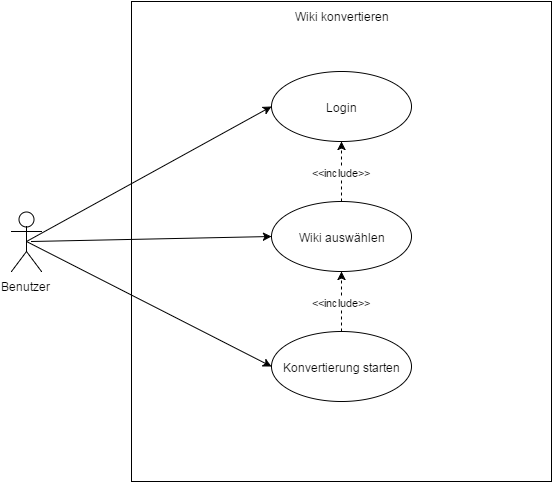
\includegraphics[width=0.85\textwidth]{images/UC_wiki_konvertieren}	
	\caption{Use-Case ''Wiki konvertieren''}
	\end{figure}
	\end{center}
	
	\subsection{Wiki bearbeiten}
	\begin{center}
	\begin{figure}
	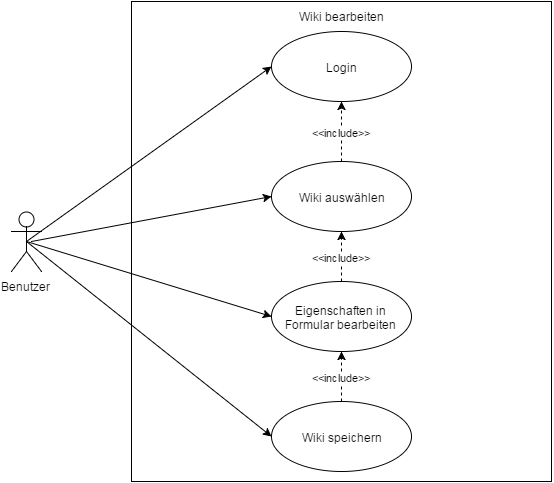
\includegraphics[width=0.85\textwidth]{images/UC_wiki_bearbeiten}	
	\caption{Use-Case ''Wiki bearbeiten''}
	\end{figure}
	\end{center}
		\newpage		
		
\end{appendices}

\end{document}